For this section we have to take into account that the mean free path of particles is proportional to their energy. Therefore, we would need too thick walls to build a lead shield that would be able to stop hard radiation, mainly cosmic radiation. Instead of trying to stop it, we have used the so-called cosmic vetos.

The cosmic veto consists of several complementary detectors, two complementary detectors for each cosmic veto in our case, with which the hard cosmic events that affect the tritium measurement will be detected and subtracted from the tritium measurement.

As you can see in Figure \ref{fig:VetoAndPrototype}, the way we have done it is to place two complementary detectors, one above the TRITIUM detector and the other below it. The distance between both vetos is set by the TRITIUM prototype, which has to be placed between both and it is $34.2~\cm$ for our latest prototype.

\begin{figure}[h]
\centering
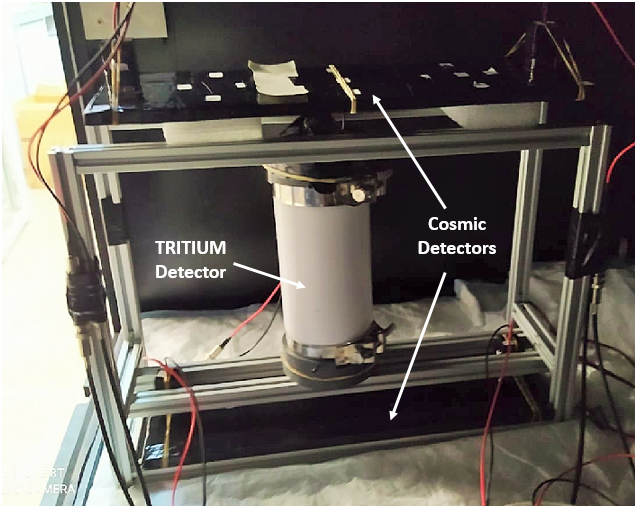
\includegraphics[scale=0.45]{3DesignPrinciples/34BackgroundRejectionSystem/Vetos_y_prototipo.png}
\caption{Cosmic veto and Tritium-IFIC 2 prototype in an aluminum mechanical structure developed by IFIC's mechanical engineering department.\label{fig:VetoAndPrototype}}
\end{figure}

We must keep in mind that we only want to eliminate the hard cosmic events that affect the tritium measurement. For that we must take into account that this cosmic veto must be placed within the lead shielding. This is because, in this case, the weak radiation, which can contribute as a false hard comic events, has been removed.

Each cosmic detector will have two photosensors, four photosensors in each cosmic veto. The most likely hard cosmic events that can affect the tritium measurement will pass through both cosmic detectors at the same time. To eliminate only them, the first thing we will do is detect only these hard cosmic events, which is achieved by reading both cosmic detectors in coincidence with the electron configuration shown in Figure \ref{subfig:ElectronicConfiguraiton4PMT} and then we will read the TRITIUM detector in anti-coincidence with the cosmic veto, that is, store the tritium measurement only when we don't detecte any hard cosmic event in the cosmic veto in time coincidence. 

In this case, if we have detect a hard cosmic event (time coincidence event in both cosmic detectors), we can be quite sure that it will cross through the tritium detector and, therefore, it will affect to their measurement, as you can see in Figure \ref{subfig:RealHardCosmicEvent}.

There is a possibility that this hard cosmic event detected in the cosmic veto comes from two different hard cosmic events (one detected in each cosmic detector as shown in Figure \ref{subfig:FakeHardCosmicEvent} but it is practically negligible.

The expected hard cosmic rate at sea level for muons, which is the main contributor of cosmic radiation at this height, is $70~\meter^{-2}\second^{-1}\steradian^{-1}$ \cite{PDG, HardCosmicMuonRate}, that is, approximately, $10^{-2}~\cm^{-2}\second^{-1}\steradian^{-1}$, as you can see in their cosmic rate plot, shown in Figure \ref{subfig:HardCoscmicRate}. If we take into account that we are doing time coincidences with signals whose width is of the order of $10~\nano\second$ we can see that the probability of obtaining two different hard cosmic events in temporal coincidence is less than $10^{-9}$ which is practically insignificant so they are not worth considering.

\begin{figure}[h]
 \centering
  \subfloat[Real hard cosmic event.]{
   \label{subfig:RealHardCosmicEvent}
    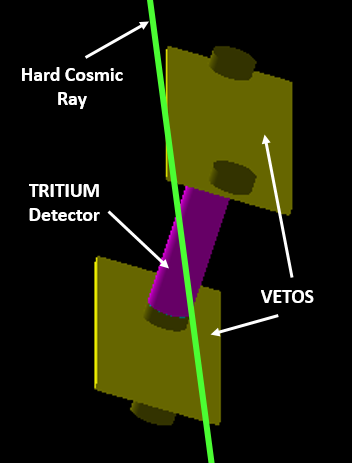
\includegraphics[width=0.25\textwidth]{3DesignPrinciples/34BackgroundRejectionSystem/Real_Event.png}}    
  \subfloat[Fake hard cosmic event.]{
   \label{subfig:FakeHardCosmicEvent}
    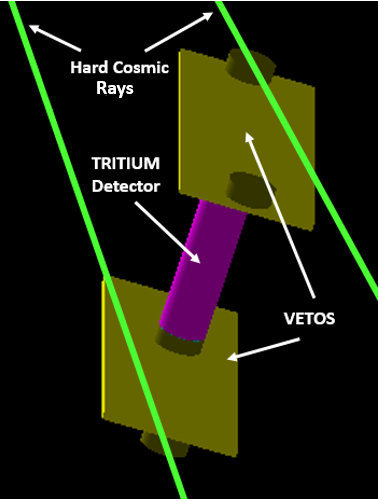
\includegraphics[width=0.25\textwidth]{3DesignPrinciples/34BackgroundRejectionSystem/Fake_Event.png}} 
    \subfloat[Hard cosmic muon rate \cite{HardCosmicMuonRatePlot}.]{
   \label{subfig:HardCoscmicRate}
    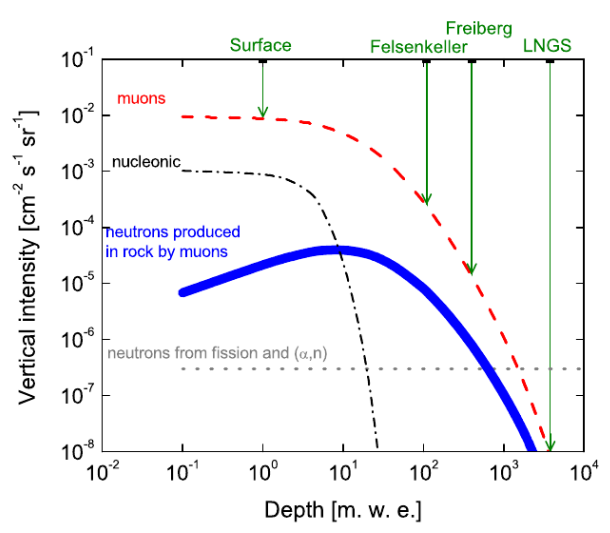
\includegraphics[width=0.42\textwidth]{3DesignPrinciples/34BackgroundRejectionSystem/HardCosmicRate.png}}     
 \caption{Hard cosmic events detected with the cosmic veto of TRITIUM: a) Affecting to the tritium measurement, b) Does not affecting to the tritium measurement. c) Hard cosmic muon rate. }
 \label{fig:HardCosmicEventsSimulation}
\end{figure}

Finally, these individual cosmic detectors, on which the cosmic veto is based, consist of a plastic scintillator block from Epic-Crystal \cite{ScintillatorVeto}, whose properties and energy emission spectrum are shown in Table \ref{tab:ParametersScintillatorVeto} and Figure \ref{fig:EmissionEnergySpectrumVeto} respectively.

\begin{table}[]
%%\centering
\begin{center}
\begin{tabular}{|c|c|c|}
%\hline
%Material & Refractive index \\
\hline \hline 
Base material & Polystyrene \\ \hline
Growth method & Polymeric \\ \hline
Density ($\gram/\cm^3$)& 1.05 \\ \hline
Refractive index & 1.58 \\ \hline
Soften temperature ($\degree$) & 75-80 \\ \hline
Light output (Anthracene) & 50-60\% \\ \hline
H/C raito & 1.1 \\ \hline
Emission peak (nm) & 415 (Blue) \\ \hline
Decay Time, (ns) & 2.4 \\ \hline
Hygroscopic & No \\ \hline
\end{tabular}
\caption{Properties of plastic scintillator blocks from Epic-Crystals. \cite{ScintillatorVeto}}
\label{tab:ParametersScintillatorVeto}
\end{center}
\end{table}

\begin{figure}[]
\centering
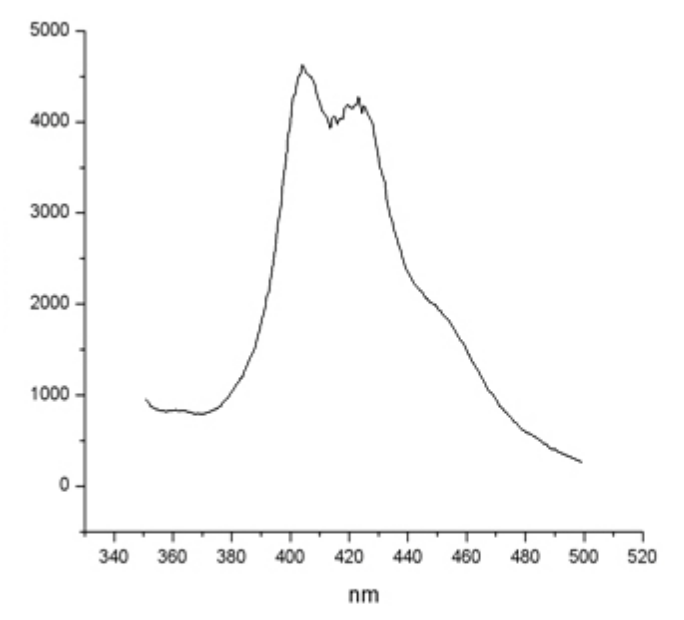
\includegraphics[scale=0.45]{3DesignPrinciples/34BackgroundRejectionSystem/EmissionEnergySpectrumVetos.png}
\caption{Emission energy spectrum of the plastic scintillation used for the cosmic vetos.\label{fig:EmissionEnergySpectrumVeto}~\cite{ScintillatorVeto}}
\end{figure}

The dimensions used are $45~\cm$ long, $17~\cm$ deep and $1~\cm$ of thickness and they are covered by three layers, teflon, aluminum and black tape, shown in Figure \ref{fig:LayersVeto}, which is used, on the one hand, to prevent external photons from reaching the scintillator plastic, giving false hard cosmic events and, on the other hand, to prevent the photons generated by the scintillator plastic from escaping before reaching the photosensor, losing real hard cosmic events.

\begin{figure}[h]
 \centering
  \subfloat[Scintillator without coating.]{
   \label{subfig:PlasticScintillatorNoCoating}
    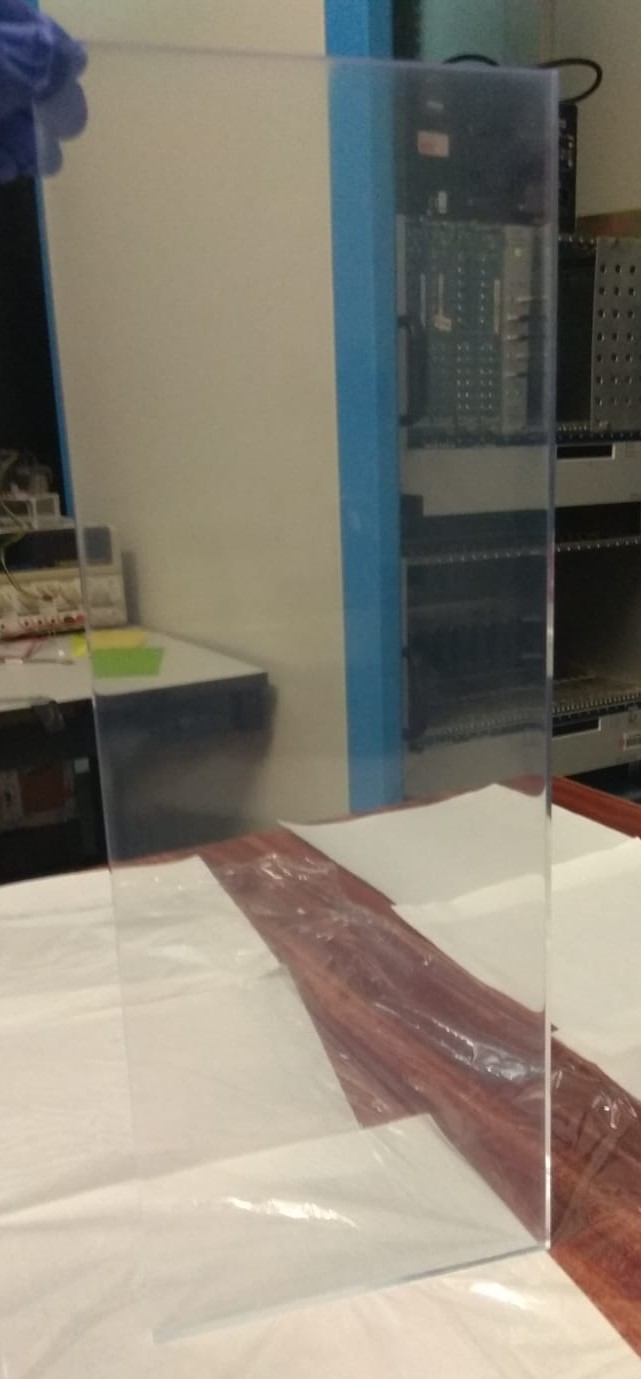
\includegraphics[width=0.23\textwidth]{3DesignPrinciples/34BackgroundRejectionSystem/NoCoating.jpeg}}    
  \subfloat[Teflon coating.]{
   \label{subfig:PlasticScintillatorTeflon}
    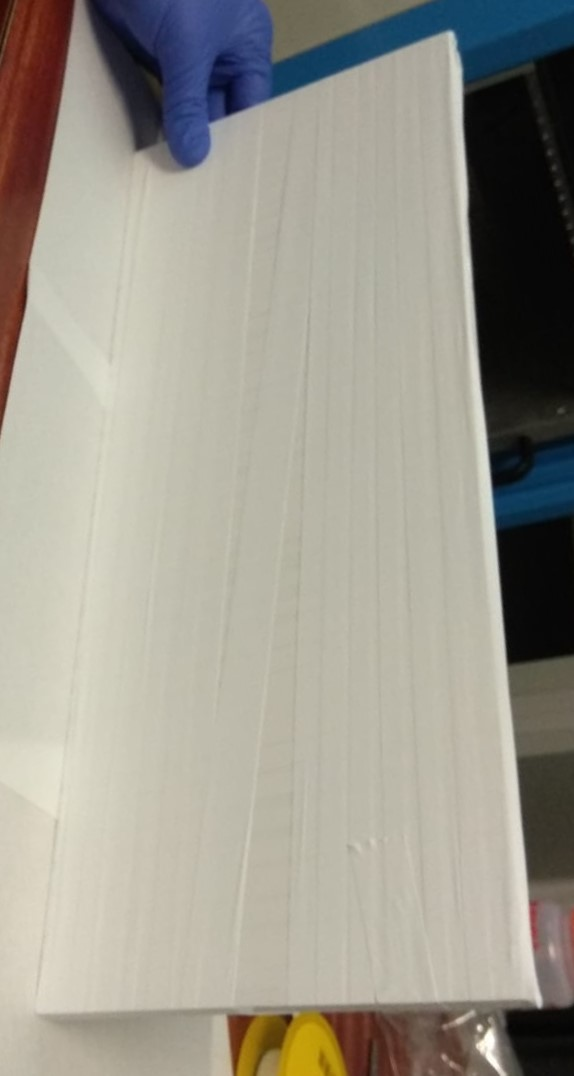
\includegraphics[width=0.23\textwidth]{3DesignPrinciples/34BackgroundRejectionSystem/TeflonCoating.jpeg}}  
  \subfloat[Aluminium coating.]{
   \label{subfig:PlasticScintillatorAluminium}
    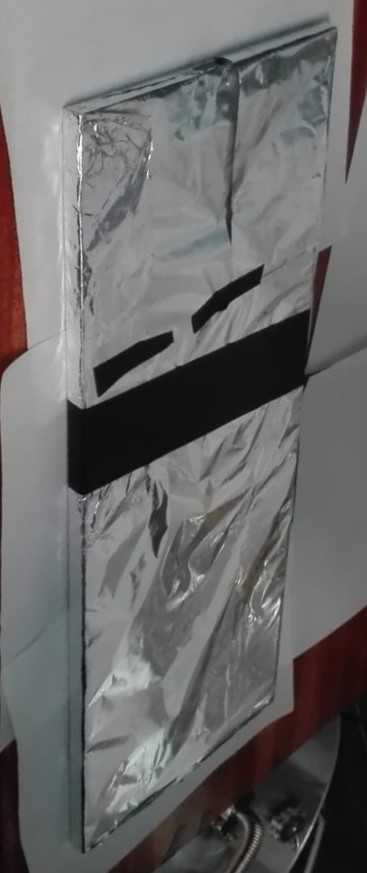
\includegraphics[width=0.23\textwidth]{3DesignPrinciples/34BackgroundRejectionSystem/AluminiumCoating.jpeg}}    
  \subfloat[Black tape coating.]{
   \label{subfig:PlasticScintillatorBlackTape}
    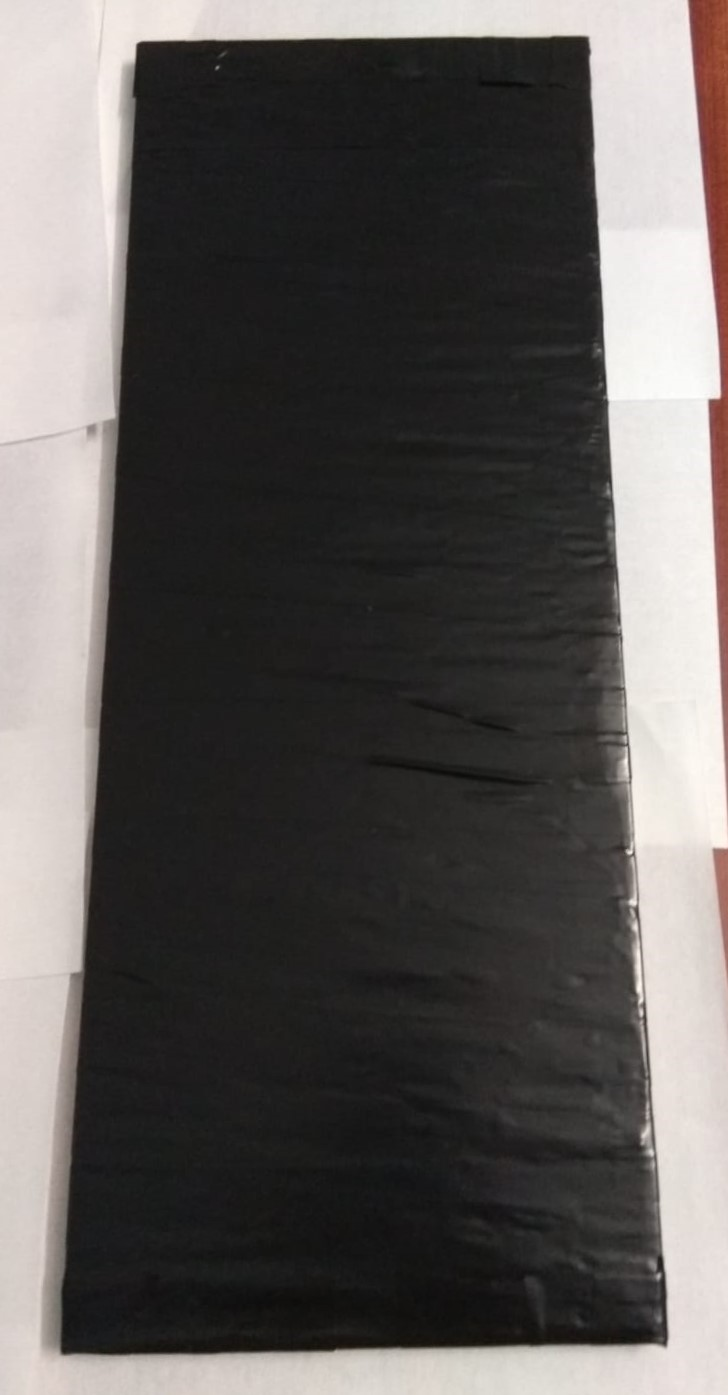
\includegraphics[width=0.23\textwidth]{3DesignPrinciples/34BackgroundRejectionSystem/BlackTapeCoating.jpeg}}
 \caption{Different layers used to cover of the cosmic veto.}
 \label{fig:LayersVeto}
\end{figure}

This coating has two $2.5\cdot{} 2.5 ~\cm^2$ windows where we can place both photosensors to read the photons produced by the plastic scintillator.

Now, we can calculate the expected hard cosmic rate for our specifically cosmic vetos. As we have seen before, the expected hard cosmic rate at sea level is $10^{-2}~\cm^{-2}\second^{-1}\steradian^{-1}$. If we take into account that, on the one hand, the solid angle of our detectors is $\omega=0.5434$, which has been calculated by integrating above the area of the TRITIUM cosmic veto, and the area of its cosmic veto is $45~\cm \cdot{} 17~\cm=765~\cm^2$, the expected hard cosmic rate on our cosmic vetos should be $2,909~$event$/\second$.